\mode<article>{As its name suggests, a PI controller consists of both a gain and an integral term. This controller is used when it is desired to improve the steady state response by increasing the system type. This controller is implemented as shown in the following block diagram}

\begin{frame}{Proportional/Integral (PI) Control}
\begin{center}
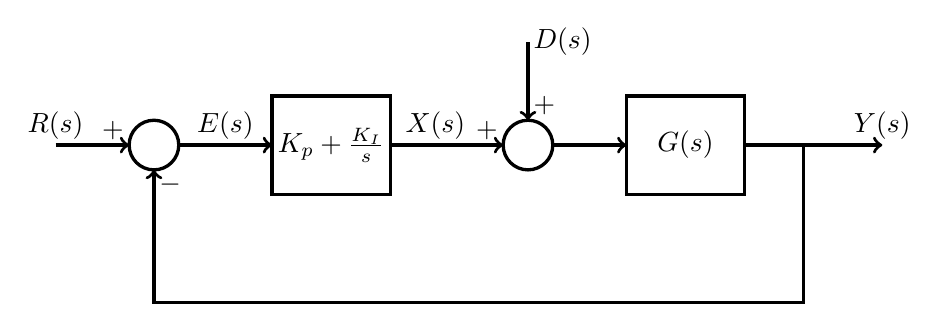
\begin{tikzpicture}[scale=1,inner sep=0pt,outer sep=0pt,very thick,
sysblock/.style={draw,rectangle,inner sep=2pt,minimum width=1.5cm,minimum height=1.25cm,very thick}]
\draw (1.25,0) node[draw,circle] (sum1) {$\rule{0pt}{18pt}$};
\draw (3.5,0) node[sysblock] (Kp) {$K_{p}+\frac{K_{I}}{s}$};
%\draw (5,0) node[draw,circle] (sum3) {$\rule{0pt}{18pt}$};
\draw (6,0) node[draw,circle] (sum2) {$\rule{0pt}{18pt}$};
\draw (8,0) node[sysblock] (G) {$G(s)$};
%\draw (8,-1.75) node[sysblock] (Kd) {$K_{d}s$};
\draw[->] (0,0) node[above=2pt] {$R(s)$} -- (sum1.180) node[above left=2pt] {$+$};
\draw[->] (sum1.0) --  node[above=2pt,pos=.5] {$E(s)$} (Kp);
%\draw[->] (Kp) -- (sum3.180) node[above left=2pt] {$+$};
\draw[->] (Kp.0) -- node[above=2pt,pos=.4] {$X(s)$}  (sum2.-180) node[above left=2pt] {$+$};
\draw[->] (sum2.0) -- (G);
\draw[->] (G) -- ++(2.5,0) node[above=2pt] {$Y(s)$};
%\draw[->] (G) ++(1.5,0) |- (Kd) -| (sum3.-90) node[below right=2pt] {$-$};
\draw[->] (G) ++(1.5,0) -- ++(0,-2) -| (sum1.-90) node[below right=2pt] {$-$};
\draw[<-] (sum2.90) node[above right=2pt] {$+$} -- ++(0,1) node[right=2pt] {$D(s)$};
\end{tikzpicture}
\end{center}
\end{frame}

\begin{example}\label{examp:PI} Let's return to the tank control problem, with a specified settling time of $\ts \leq 0.2$ s, but now $0$ steady state error for a unit step reference input. In order to meet these specifications with a proportional controller, we would need to apply infinite gain, so we instead turn to a PI control

\begin{frame}
\begin{center}
\input{Graphics/tankandvalvemeasPI}
\end{center}
\end{frame}
which has block diagram

\begin{frame}
\begin{center}
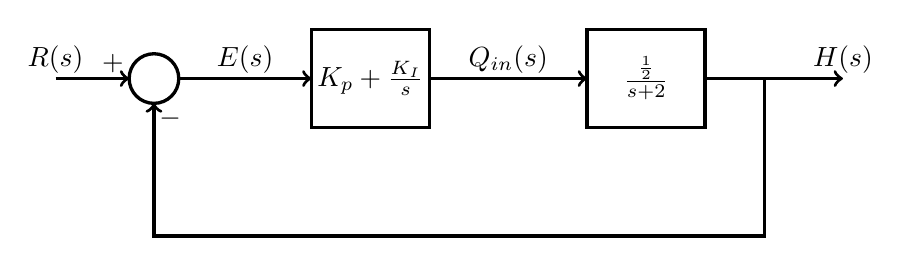
\begin{tikzpicture}[scale=1,inner sep=0pt,outer sep=0pt,very thick,
sysblock/.style={draw,rectangle,inner sep=2pt,minimum width=1.5cm,minimum height=1.25cm,very thick}]

\draw (1.25,0) node[draw,circle] (sum1) {$\rule{0pt}{18pt}$};
\draw (4,0) node[sysblock] (Kp) {$K_{p}+\frac{K_{I}}{s}$};
\draw (7.5,0) node[sysblock] (G) {$\frac{\frac{1}{2}}{s+2}$};

\draw[->] (0,0) node[above=2pt] {$R(s)$} -- (sum1.180) node[above left=2pt] {$+$};
\draw[->] (sum1.0) --  node[above=2pt,pos=.5] {$E(s)$} (Kp);
\draw[->] (Kp) -- node[above=2pt] {$Q_{in}(s)$} (G);
\draw[->] (G) -- ++(2.5,0) node[above=2pt] {$H(s)$};
\draw[->] (G) ++(1.5,0) -- ++(0,-2) -| (sum1.-90) node[below right=2pt] {$-$};
\end{tikzpicture}
\end{center}
\end{frame}
\begin{frame}
The closed loop transfer functions are
\begin{align*}
\frac{H(s)}{R(s)} &= \frac{\frac{K_{p}}{2}s+\frac{K_{I}}{2}}{s^2+\frac{4+K_{p}}{2}s+\frac{K_{I}}{2}}\\
\frac{E(s)}{R(s)} &= \frac{s^2+2s}{s^2+\frac{4+K_{p}}{2}s+\frac{K_{I}}{2}}
\end{align*}
Note that since $E(s)/R(s)$ has a zero at $s=0$, we automatically meet the steady state error specification, as
\[
e_{ss} = \lim_{s\rightarrow 0}s\frac{s^2+2s}{s^2+\frac{4+K_{p}}{2}s+\frac{K_{I}}{2}}\frac{1}{s} = 0
\]
We need only choose $K_{p}$ and $K_{I}$ to meet our settling time specification. 
\end{frame}
\begin{frame}
\mode<presentation>{\begin{center}
$\frac{H(s)}{R(s)} = \frac{\frac{K_{p}}{2}s+\frac{K_{I}}{2}}{s^2+\frac{4+K_{p}}{2}s+\frac{K_{I}}{2}}$
\end{center}}
Since $2\zeta\omega_{n} =\frac{4+K_{p}}{2}$, $\zeta\omega_{n} = 1+\frac{K_{p}}{4}$. Thus, we require
\[
\ts =\tseqtwo =  \frac{4.6}{1+\frac{K_{p}}{4}} \leq 0.2
\]
so we should choose
\[
K_{p}\geq 88
\]
$K_{I}$ can be chosen as desired. For example, we may wish to have a reasonable damping ratio.
\end{frame}
\begin{frame}
\mode<presentation>{\begin{center}
$\frac{H(s)}{R(s)} = \frac{\frac{K_{p}}{2}s+\frac{K_{I}}{2}}{s^2+\frac{4+K_{p}}{2}s+\frac{K_{I}}{2}}$
\end{center}}
From above,  $\zeta= \frac{1+\frac{K_{p}}{4}}{\omega_{n} }$, and from $\frac{H(s)}{R(s)}$, $\omega_{n} =\sqrt{\frac{K_{I}}{2}}$.  With $K_{p}=88$, 
\[
\zeta = \frac{(1+88/4)}{\omega_{n}} = \frac{23}{\sqrt{K_{I}/2}}
\]
So $K_{I} = 4232$ will give a damping ratio of $0.5$.
\end{frame}
\end{example}

